\chapter{METHODOLOGY}
{\baselineskip=2\baselineskip
	
	In this chapter, we detail the methodology employed to conduct the study, providing a comprehensive overview of the research design, data collection, and analytical procedures.
	
	\section{Research Design}
	Your research design.
	
	\section{Tables}
	
	\begin{table}[ht]
		\centering
		\caption{Sample Data Table}
		\label{tab:sample}
		\begin{tabular}{l c r}
			\toprule
			\textbf{Item} & \textbf{Quantity} & \textbf{Price (\$)} \\
			\midrule
			Apples & 10 & 0.50 \\
			Bananas & 5 & 0.30 \\
			Cherries & 20 & 1.20 \\
			Dates & 50 & 2.50 \\
			\bottomrule
		\end{tabular}
	\end{table}
	
	\section{Images}
	\begin{figure}
		\centering
		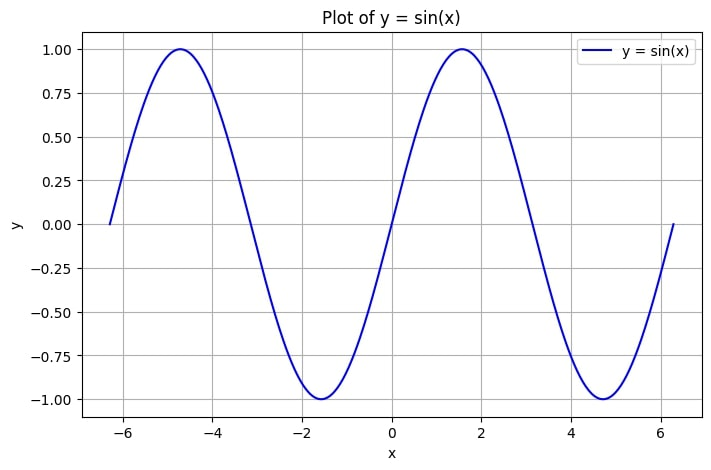
\includegraphics[width=0.7\linewidth]{figures/sinegraph}
		\caption{Sine Graph}
		\label{fig:sinegraph}
	\end{figure}
	
	\begin{figure}[h]
		\centering
		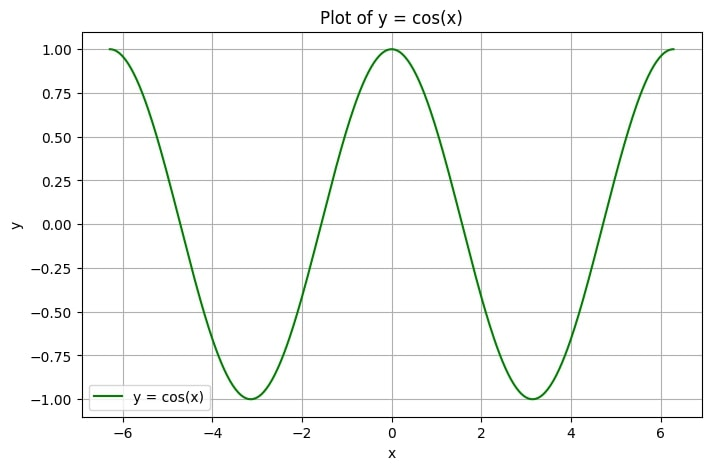
\includegraphics[height=0.3\textheight]{figures/cosinegraph}
		\caption[Cosine Graph]{Cosine Graph}
		\label{fig:cosinegraph}
	\end{figure}
}
